\chapter{The Nitrogen-Vacancy center in Diamond}
The nitrogen-vacancy (NV) center in diamond provides a natural occurring qubit register in a solid state environment.
This chapter will explain how the electronic and nuclear spins can be initialized, controlled and read-out using optical and microwave pulses.

The methods described in this chapter are limited to nuclear spins for which spin transitions can be addressed selectively.
The addressing of spins for which the spin transitions cannot be readily resolved will be discussed in \cref{chap:addressing_weakly_coupled_carbons}.

\section{The electronic spin}
The NV-center is a naturally occurring impurity in diamond consisting of a substitutional nitrogen and an adjacent lattice vacancy (\cref{fig:Sil_Robledo}).
The NV-center can be in a neutral charge state ($\mathrm{NV}^0$) or in a negatively charged state ($\mathrm{NV}^-$).
In this thesis we are mainly interested in the negatively charged state, where an additional electron is captured from the environment.
For the $\mathrm{NV}^-$ the ground state is a spin-triplet that forms the basis of our qubit.

The electronic ground state can be described by the Hamiltonian \citep{Bernien2014Control}:
 \begin{equation}
H_\mathrm{GS} = \Delta {{S}_\mathrm{z}}^2 + \gamma_e \bm{B} \cdot \bm{S}
\end{equation}
Where $\bm{S}_i$ are the Pauli-spin operators,  $\gamma_e  = 2.802\,\mathrm{ MHz/G}$  the electron gyro-magnetic ratio and $\Delta \approx 2.88\, \mathrm{GHz}$ the zero-field splitting.
In this expression the interactions with the nitrogen nucleus and the carbon spin bath are not included.
In the experiments a magnetic field $B_z = 304\,\mathrm{G}$ is applied along the NV-axis\footnote{The NV-axis is the axis going trough both the nitrogen and the vacancy. }.
The magnetic field lifts the degeneracy of the $m_s = \pm 1$.

In this thesis we define our electronic qubit  as the two level system  $m_s=0:=|0\rangle$ and $m_s = +1 := |1\rangle$.

\begin{figure}[htbp]
    \centering
    \begin{subfigure}[t]{0.49\textwidth}\centering
        \caption{}
        \label{fig:Sil_Robledo}
        \includegraphics[scale = 1.4]{Img/Sil_Robledo.pdf}
    \end{subfigure}
    \begin{subfigure}[t]{0.49\textwidth}\centering
       \caption{}
       \label{fig:readoutRobledo}
       \includegraphics[scale = 1.4]{Img/readout_Robledo.pdf}
   \end{subfigure}
   \caption{\textbf{\subref{fig:Sil_Robledo}} Scanning electron microscope image of a solid immersion lens (SIL) similar to those used in the experiments. Overlaid sketch shows a schematic representation of the NV-center. Inset shows a confocal microscope image of an NV-center similar to those used in the experiments. Figure from \citet{Robledo2011HighFidelity}.  \textbf{\subref{fig:readoutRobledo}}, Energy levels used for initialization and readout of the electronic-spin state. Figure from \citet{Robledo2011HighFidelity}}
\end{figure}

\subsection{Initialization and readout of the electronic-spin state}
The transitions between the electronic ground-state and excited state are spin dependent and lie in the optical domain ($\sim 637\, \mathrm{ nm}$).
At low temperatures these transitions can be resonantly excited.
For this reason, experiments were performed at cryogenic temperatures ($4\,\mathrm{K}$).
The exact frequencies of these transitions depend on magnetic field and strain \citep{Hensen2011MeasurementBased}.

\Cref{fig:readoutRobledo} shows the optical transitions used to initialize and read-out the electronic spin.
The $E'$ transition excites both the $m_s =+1$ and the $m_s=-1$ states to the excited state.
The $E_\mathrm{x}$ transition excites the $m_s = 0$ state to the excited state.
There is a small probability that the spin is flipped in an optical cycle, denoted by the dashed line.

By cycling an optical transition the spin state can be read-out and initialized \citep{Robledo2011HighFidelity}.
By applying a pulse to the $E_x$ transition a photon can be detected when the state falls back to the ground state.
Because the $E_x$ only excites the $m_s=0$ state photons can only be detected when the system is in the $\ket{0}$-state.

By pumping one of these transitions the spin can be initialized.
Pumping will cause the population to cycle between the ground and excited state with a small probability of the spin flipping.
When the spin flips it ends up in the state that is not being excited and stays there.

Because the number of pumping cycles before the spin flips is limited, the fidelity with which the spin can be read-out is limited by the detection efficiency of the emitted photons.
A solid immersion lens (SIL), visible in \cref{fig:Sil_Robledo}, is milled onto the sample to maximize the detection efficiency.

Using these methods a readout fidelity of $F= 90.55 \pm 0.40 \%$ can be reached.

\subsection{Controlling the electronic-spin state}
The state of a qubit can be represented as a vector on the Bloch-sphere where the $\ket{0}$-state lies at the north pole and the $\ket{1}$-state at the south pole.
The state vector rotates around the quantization-axis with a frequency depending on the energy splitting between the two states: the Larmor frequency.
For the NV-electronic spin the quantization axis points in the z-direction (towards $\ket{0}$) and the  Larmor frequency is given by \cref{eq:larmor_electronic_spin}:
\begin{equation}
    \omega_L =\Delta + \gamma_e {B_\mathrm{z}}
    \label{eq:larmor_electronic_spin}
\end{equation}


By applying an external field a term is added to the Hamiltonian, the quantization-axis is changed, thereby changing its evolution.
By applying microwaves with a frequency equal to $\omega_L$ the transition between $\ket{0}$ and $\ket{1}$ can be driven \citep{Jelezko2004Observation}.
Resonant microwave pulses are applied to the sample trough an on-chip gold stripline, visible in \cref{fig:Sil_Robledo} as the light area just below the SIL.

\section{Controlling nuclear spins}
The electronic-spin interacts with each nuclear spins in its environment trough the hyperfine interaction, which is dependent on their position.
Dependent on the strength of the hyperfine interaction close by spins can be controlled directly by applying microwave pulses.

\subsection{The Hyperfine Interaction}
The coupling between the electronic spin of the NV-center and a nuclear-spin is given by the hyperfine-interaction.
The hyperfine interaction is a spin-spin interaction.

For nuclear spins the Hamiltonian therefore depends on the electronic spin-state of the NV-center.
For a magnetic field ($B_\mathrm{z}$) in the z-direction the Hamiltonian is given by \cref{eq:nuclear_hamiltonian_0,eq:nuclear_hamiltonian_1} \citep{Taminiau2014Universal}:
\begin{equation}
    \label{eq:nuclear_hamiltonian_0}
    H_0= -Q I_{\mathrm{z}}^2+ \gamma_{n} B_\mathrm{z} I_\mathrm{z}
\end{equation}
\begin{equation}
    \label{eq:nuclear_hamiltonian_1}
    H_1 = -Q I_{\mathrm{z}}^2+\gamma_{n} B_\mathrm{z} I_\mathrm{z} +H_{\mathrm{HF}}
\end{equation}
Corresponding respectively to the electronic spin being in the $m_s = 0$ and in the $m_s = +1$ state.
Where $\bm{I}$ and $\bm{S}$ are the nuclear and electronic spin operators, $\gamma_n$ is the gyro-magnetic ratio of the nucleus and $Q$ is the nuclear quadrupole splitting.
The quadrupole term is $Q= 2\pi \cdot 4.946 \,\mathrm{ MHz}$ for the nitrogen spin \citep{Bernien2014Control}.
The quadrupole term is not present for carbon-13 spins.


The Larmor frequency for a nucleus is given by  \cref{eq:nuclear_larmor}:
\begin{equation}
\label{eq:nuclear_larmor}
{\omega_L} =-Q{I}_{\mathrm{z}}^2+ \gamma_{n}B_\mathrm{z}
\end{equation}

\subsection{Controlling the nitrogen nuclear spin}
\label{sec:nitrogen_spin_control}
The nitrogen-spin adjacent to the vacancy can be controlled using the hyperfine interaction.
Because both the zero-field splitting $\Delta$ of the electronic-spin is much larger than the hyperfine coupling between the nuclear and electronic spin ($A_\mathrm{N} = 2\pi \cdot 2.186 \, \mathrm{MHz} $), the secular approximation can be used, leading to the following system Hamiltonian:
\begin{equation}
        H_\mathrm{GS} = \Delta {{S}_\mathrm{z}}^2 + \gamma_e \bm{B} \cdot \bm{S} -Q I_{\mathrm{z}}^2+\gamma_{n} B_\mathrm{z} I_\mathrm{z} - A_\mathrm{N} S_z\cdot {I_z}
\end{equation}

The hyperfine interaction between the nitrogen and electronic spin causes the transition between $m_s=0$ and $m_s =1$ to be split.
This magnitude of the splitting is equal to $A_N$ and  is clearly resolved in the Electron Spin Resonance (ESR) shown in the top panel of \cref{fig:HF_split_levels}.


    \begin{figure}[htbp]
    \centering
        \begin{tikzpicture}
            \node[anchor=south west,inner sep=0] at (0,0) {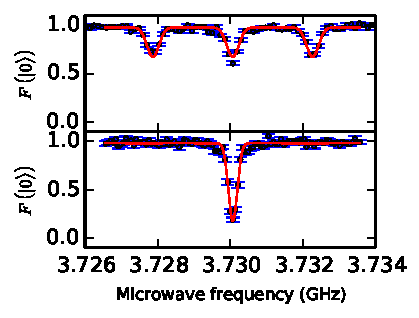
\includegraphics{Img/DarkESR_2.pdf}};
            \node (A) at (2.6,4.4) {};
            \node (B) at (3.92,4.4) { };
            \node (C) at (5.3,4.4) { };
            \draw[latex-latex, font=\small] (A) -- node[label =270: $A_\mathrm{N}$] {} (B);
            \draw[latex-latex, font=\small] (B) -- node[label =270: $A_\mathrm{N}$] {} (C);
        \end{tikzpicture}
        \caption{ Electron Spin Resonance (ESR) for uninitialized (top) and initialized nitrogen spin (bottom) of the $m_s =0 \rightarrow m_s = +1$ transition. In the ESR the spin is prepared in $\ket{0}$, a microwave pulse is applied and the electron is read out.
        The microwave frequency is swept.
        When the microwave is on resonance the spin will be rotated out of $\ket{0} $ and a decrease will be visible in the signal.
        In the top figure the transition is split due to the interaction with the NV's nitrogen nuclear spin.
        In the lower figure the nitrogen spin state is initialized and the splitting disappears.}
        \label{fig:HF_split_levels}
    \end{figure}

The hyperfine interaction can be used to measure the nitrogen's spin state.
Every time an experiment is started the nitrogen starts out in a mixed state.
This means that every time an uninitialized nitrogen is measured it is equally likely to end up in one of its three states, as can be seen in the top panel of \cref{fig:HF_split_levels}.
The nitrogen state can be measured by initializing the electron in the split $m_s = +1$ state and driving one of the transitions to $m_s=0$.
Only if the nitrogen was in the state corresponding to the transition being driven will a measurement of the $m_s =0$ state give a positive result.

By resetting and repeating this procedure until a positive result is measured the nitrogen-spin can be initialized.
The electronic spin-state can be reset by applying a resonant laser as shown in the previous section.
The nuclear spin-state can be reset by applying two resonant lasers resonant with $E_x$ and $E'$.

This procedure is known as measurement based initialization (MBI) and is used in our experiments.
The lower panel of \cref{fig:HF_split_levels} shows an ESR after the nitrogen has been initialized using MBI.

\subsection{Hyperfine coupling of carbon-13 spins}
For carbon-13 spins the hyperfine term ($H_{\mathrm{HF}}$) of \cref{eq:nuclear_hamiltonian_1} consists of a contact term and a dipole term.
The contact term results from an overlap between the electronic- and nuclear- wave-functions.
The contact term is negligible for all but the carbon-spins closest to the NV-center.
For close-by carbon spins hyperfine couplings have been  calculated \citep{Gali2008Ab,Gali2009Identification} and measured \citep{Smeltzer201113}.

For carbons where the contact term is negligible the dipole term is dominant and is given by \cref{eq:dipole_component_of_hyperfine} \citep{Lange2012Quantum}:
\begin{equation}
\label{eq:dipole_component_of_hyperfine}
H_{\mathrm{dip}} = \frac{\mu_0 \gamma_e \gamma_{\mathrm{C}} \hbar^2 }{4 \pi r^3} [ \bm{S \cdot I} - 3 (\bm S \cdot \hat{\bm{n}}_{\mathrm{HF}})(\bm I \cdot \hat{\bm{n}}_{\mathrm{HF}})]
\end{equation}
Where $\hat{\bm{n}}_{\mathrm{HF}}$ is a unit vector pointing from the electronic spin to the nucleus, $r$ is the distance between the electronic and nuclear spin, and $\mu_0$ the magnetic constant.
The dipole term can be split into a parallel and orthogonal component such that:
\begin{equation}
     H_{\mathrm{HF}} = A_\parallel I_\mathrm{z} + A_\perp I_x
 \end{equation}


From \cref{eq:dipole_component_of_hyperfine}  the parallel and orthogonal components of the hyperfine interaction, with respect to the NV-axis along the z-direction, can be derived to be:
 \begin{align}
A_\parallel= - \frac{\mu_0 \gamma_e \gamma_{\mathrm{C}} \hbar^2 }{4 \pi r^3} \left(3\cdot \frac{z^2}{r^2}-1\right)\\
 A_\perp =  -\frac{\mu_0 \gamma_e \gamma_{\mathrm{C}} \hbar^2 }{4 \pi r^3}\left( 3\cdot\frac{\sqrt{x^2+y^2}\cdot z}{r^2}\right)
\end{align}


\subsection{Strongly coupled spins}
Carbon spins can be controlled using the methods described in \cref{sec:nitrogen_spin_control} when it is possible to selectively address its spin-dependent transitions.
When two transitions can be resolved in an ESR they can be addressed by applying microwave pulses of the corresponding frequencies.
However if two transitions overlap in an ESR, applying a microwave pulse at the corresponding frequency will address both transitions.

Two transitions cannot be resolved when the splitting between them is smaller than the width of the transition.
The magnitude of the splitting is determined by the strength of the interaction and the broadening of the transitions is caused by decoherence.
We define a spin to be strongly coupled when it is possible to readily resolve it's transitions in an ESR experiment with negligible power broadening.
Conversely a spin is weakly coupled when it is not possible to readily resolve its transitions in an ESR.

Using the methods described in \cref{sec:nitrogen_spin_control} strongly-coupled carbon-13 spins have been controlled and initialized \citep{Robledo2011HighFidelity}.

The next section will explain what decoherence is and how it relates to the broadening of transitions.
The next chapter will discuss how spins for which transitions cannot be resolved can be addressed trough dynamical decoupling.

\section{Decoherence}
The ESR signal is broadened because the NV-center interacts with the spin bath in its environment.
The spin bath consists of spins that are coupled to the NV-center.
Just like the uninitialized nitrogen spin these are in a mixed state.
This means that for every iteration of an experiment the spin bath can have a different configuration.
These different configurations of the spin bath slightly shift the addressed electron transition causing the broadening of the transition.

\subsection{Decoherence time}
The variations in the spin-bath configuration can be measured with a Ramsey experiment.
In a Ramsey experiment (\cref{fig:Ramsey_gijs}) the electronic spin is brought into a superposition between the $\ket{0}$ and $\ket{1}$-state where it freely evolves for a time $\tau$.
Provided the oherent uperpsition is preserved, a final pulse brings the state back into $\ket{0}$ where it is read out.

By applying a slight detuning to the rotating frame used to keep the phase fixed an oscillation can be seen in the signal (\cref{fig:electron_T2*}).
Due to the different spin-bath configurations the evolution frequency varies slightly between experiments, this causes the measured signal to decay as the different oscillations move out of phase with each other.
The decay is known as decoherence and the $1/e$-time of the decay is known as the decoherence time $T_2^*$.
For a Ramsey experiment the decay follows a Gaussian profile \cref{eq:Ramsey_decay}:
\begin{equation}
    K(\tau) = e^{-(\tfrac{\tau}{T_{2}^*})^n}
    \label{eq:Ramsey_decay}
\end{equation}
Where $K$ is the amplitude and $n =2$ for a Gaussian profile.
The $T_2^*$ of the NV-electron spin used in this thesis was measured to be $T_{2,e}^* = 4.54 \pm 14\, \mu\mathrm{s}$ with initialized nitrogen-spin.
The decay follows a Gaussian profile within two $\sigma$: $n = 1.81 \pm 0.14$.

\begin{figure}[htbp]
    \centering
    \begin{subfigure}[t]{0.49\textwidth}\centering
        \caption{}
        \includegraphics{Img/Ramsey_Gijs.pdf}
        \label{fig:Ramsey_gijs}
    \end{subfigure}
    \begin{subfigure}[t]{0.49\textwidth}\centering
        \caption{}
        \includegraphics{Img/electron_T2star.pdf}
        \label{fig:electron_T2*}
    \end{subfigure}
        \caption{
        \textbf{\subref{fig:Ramsey_gijs}} schematic representation of a Ramsey experiment. Figure from \citet{Lange2012Quantum}.
        In a Ramsey experiment a qubit is brought into the $xy$-plane by a $\pi/2$-pulse where it evolves freely for a time $\tau$ before being subjected to a final $\pi/2$ pulse to read out its $x$-component.
        By applying a detuning ($\omega_d$) to the rotating frame the spin will pick up a phase $\phi = \omega_d \tau$ during free evolution.
        The final pulse will rotate the spin towards the poles depending on the phase picked up during free evolution.
        This manifests itself as an oscillation.
        Because the configuration of the spin-bath is slightly different between experiments the frequency of the oscillation will vary with each iteration.
        This variation in frequency between iterations will cause the oscillation to decay.
        \subref{fig:electron_T2*} shows a Ramsey experiment for the electronic spin.
        The $y$-axis shows the fidelity of the measured state to the $\ket{0}$-state of the electronic spin.
        A $T_{2,e}^*$ of $4.54 \pm 0.14\, \mu\mathrm{s}$ was measured for the electronic spin. The decay follows a Gaussian profile within uncertainty $n = 1.81 \pm 0.14$. }
\end{figure}


\subsection{Relation between decoherence and transition broadening}
The decay in a Ramsey experiment is a measure for variations of the spin-bath in the time-domain while the broadening of transitions in an ESR is a measure for variations of the spin-bath in the frequency domain.
The decay of the Ramsey and the shape of the ESR for negligible power broadening are related trough a Fourier transform and described by \cref{eq:ESR_dip_shape} :
\begin{equation}
    \mathcal{F} \{ K(\tau) \} =  C e^{-\tfrac{(2\pi \cdot f) ^2 \cdot T_{2e}^{*2}}{ 4}}
    \label{eq:ESR_dip_shape}
\end{equation}
Where $C$ is a normalization constant.
Because the decay of the Ramsey is Gaussian the shape of a transition in the ESR is also Gaussian.

Two identical Gaussians can be readily resolved when the separation between their maxima is larger than their full-width-half-maximum (FWHM).
The FWHM (in Hz) of the ESR is given by \cref{eq:FWHM}:
\begin{equation}
    \mathrm{FWHM} =  \frac{2\sqrt{\ln{2}}}{\pi T_{2e}^*}
    \label{eq:FWHM}
\end{equation}

An estimation of when carbon spins can be resolved is given by the strength of the hyperfine interaction.
At low magnetic field ($\gamma_e B \ll A$) the splitting caused by a carbon spin is equal to the total interaction strength $A$.
At high field ($\gamma_e B \gg A$) the secular approximation is valid and the splitting is equal to the parallel component of the hyperfine $A_\parallel$.
We can readily resolve a transition when the shift due to the corresponding interaction is larger than the FWHM of the transition.

At a natural concentration of carbon-13 spins ($\mu =1.1\%$) NV-centers have a typical  electron $T_{2e}^* \approx 2\,\mu \mathrm{s}$ at low field that depends on the exact configuration of the spin-environment.
Increasing the carbon-13 concentration generally reduces $T_{2e}^*$.
On the sample used for the experiments $T_{2e}^*=4.54 \pm 0.14\, \mu\mathrm{s}$ was measured at $304\, \mathrm{G}$
This means that the hyperfine coupling must be larger than $2\pi\cdot 265\,\mathrm{kHz}$ in a typical NV-center, and larger than $2\pi\cdot 117\, \mathrm{kHz}$ in the sample used in this thesis for a carbon to be strongly coupled.

As the presence of strongly coupled carbons close to the NV-center is governed by probability and the probability of getting 3-5 strongly coupled carbons is very low it is necessary to develop methods to address weakly coupled carbons.
The next chapter will demonstrate methods to extend the coherence time and address weakly coupled carbons, thereby enlarging the spin-register.

